\subsection{Quantizador}
% 
\begin{questions}
\question{
Na conversão analógico-digital é utilizado um quantizador $Q$. O quantizador
mapeia os valores de sua entrada $X$ em um conjunto finito de valores (níveis 
de quantização) $Y \in \{y_1, y_2, \ldots, y_N \}$.
Como podemos determinar a informação mútua $I(X;Y)$ conhecendo a distribuição 
da saída $Y$? É possível utilizar $I(X;Y)$ para determinar a entropia de $X$?
Justifique sua resposta.

\begin{figure}[!ht]
  \centering
    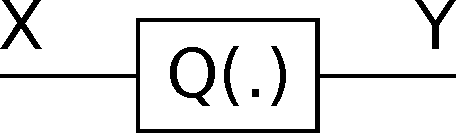
\includegraphics[width=0.25\textwidth]{../images/quantizador.pdf}
  \caption{Quantizador.}
  \label{fig:quantizador}
\end{figure}
}

\begin{solution}
  Como a saída $Y$ é uma função de $X$, $Y = Q(X)$, teremos que a incerteza sobre $Y$
  dado $X$ será nula, $H(Y|X) = 0$. Desta forma, teremos
  \begin{eqnarray}
  I(X;Y) &=& H(Y) - \underbrace{H(Y|X)}_{=0} \nonumber \\
        &=& H(Y) \nonumber \\
        &=& - \sum_{y \in \mathcal{Y}} p(y) \log p(y)
  \end{eqnarray}
  Conhecendo a distribuição $p(y)$ poderemos calcular a informação mútua $I(X;Y)$.

  Por outro lado, não podemos afirmar que $X$ é uma função de $Y$ (de forma geral, isto não ocorrerá),
  assim $H(X|Y)$ não será nula e não teremos como determinar $H(X)$ conhecendo apenas $p(y)$.

\end{solution}
\end{questions}
